
\begin{center}
\Huge
	Funktionsegenskaber
\end{center}
\section*{Surjektivitet og injektivitet}
\stepcounter{section}

\begin{defn}[Surjektiv funktion]
Lad $f:A \to B$ være givet. Hvis billedet af $A$ under $f$ opfylder, at 
\begin{align*}
f(A) = B, 
\end{align*}
så siger vi, at $f$ er \textit{surjektiv}. 
\end{defn}
Hvis $f(A) = B$, så betyder det, at værdimængden for $f$ er lig dispositionsmængden for $f$, altså at Vm$(f) = B.$ Funktionen kan altså ramme alt i dispositionsmængden. 
\begin{exa}
Funktionen $f:\mathbb{R} \to \mathbb{R}$ givet ved
\begin{align*}
f(x) = 2x+3
\end{align*}
er surjektiv, da $f(x)$ kan antage alle reelle tal som værdi.
\end{exa}
\begin{exa}
Funktionen $f:\{1,\hdots,4\} \to \{1,\hdots,5\}$, der ses af Figur \ref{fig:ikkesur} er ikke surjektiv, da elementet $1\in \{1,\hdots,5\}$ ikke ligger i værdimængden for $f$. Derimod er funktionen $g: \{1,\hdots,4\} \to \{1,2,3\}$ er surjektiv, da alle elementer i dispositionsmængden rammes af $g$.
\begin{figure}[H]
\centering
\begin{tikzpicture}
\node at (1,0.6) {$f$};
\node at(0,0) (1) {1};
\node at(0,-1) (2) {2};
\node at(0,-2) (3) {3};
\node at(0,-3) (4) {4};
\node at (2,-0) (5) {1};
\node at (2,-1) (6) {2};
\node at (2,-2) (7) {3};
\node at (2,-3) (8) {4};
\node at (2,-4) (9) {5};
\draw[-{To[scale = 1.3]}] (1) -- (6);
\draw[-{To[scale = 1.3]}] (2) -- (7);
\draw[-{To[scale = 1.3]}] (3) -- (8);
\draw[-{To[scale = 1.3]}] (4) -- (9);
\node at (6,0.6) {$g$};
\node at(5,0) (10) {1};
\node at(5,-1) (20) {2};
\node at(5,-2) (30) {3};
\node at(5,-3) (40) {4};
\node at (7,-0) (50) {1};
\node at (7,-1) (60) {2};
\node at (7,-2) (70) {3};
\draw[-{To[scale = 1.3]}] (10) -- (50);
\draw[-{To[scale = 1.3]}] (20) -- (50);
\draw[-{To[scale = 1.3]}] (30) -- (60);
\draw[-{To[scale = 1.3]}] (40) -- (70);
\end{tikzpicture}
\caption{Diagram for funktionerne $f$ og $g$.}
\label{fig:ikkesur}
\end{figure}
\end{exa}

\begin{defn}[Injektiv funktion]
	Lad $f:A \to B$ være givet. Hvis det for to elementer $f(x_1)\in B$ og $f(x_2)\in B$ i 		    værdimængden for $f$ gælder, at
	\begin{align*}
		f(x_1) = f(x_2) \ \Rightarrow \ x_1 = x_2,
	\end{align*}	 
	så siges $f$ at være \textit{injektiv}. 
\end{defn}
At $f$ er injektiv betyder, at to forskellige værdier i definitionsmængden for $f$ nødvendigvis bliver sendt til to forskellige værdier i værdimængden for $f$.
\begin{exa}
	Lad $f:\mathbb{R} \to \mathbb{R}_{\geq 0}$ være givet ved
	\begin{align*}
	f(x) = x^2.
	\end{align*}
	Denne funktion er ikke injektiv, da der til hver funktionsværdi $f(x)$ tilhører to $x$-værdier - $x$ og $-x$. Det er 	eksempelvist opfyldt, at $f(2) = f(-2) = 4$. 
\end{exa}
\begin{exa}
	Funktionen $f: \{1,\hdots,4\} \to \{1,\hdots, 5\}$, der ses på Figur \ref{fig:inj}
	 er injektiv,  da der kun er én pil hen til hvert
	punkt i $B$, hvorimod
	 $g:\{1,\hdots,4\} \to \{1,\hdots, 5\}$ er ikke injektiv,da to pile peger hen til punkterne $1,4\in \{1,\hdots,4\}$.
	\begin{figure}[H]
		\centering
		\begin{tikzpicture}
			\node at (1,0.6) {$f$};
			\node at(0,0) (1) {1};
			\node at(0,-1) (2) {2};
			\node at(0,-2) (3) {3};
			\node at(0,-3) (4) {4};
			\node at (2,-0) (5) {1};
			\node at (2,-1) (6) {2};
			\node at (2,-2) (7) {3};
			\node at (2,-3) (8) {4};
			\node at (2,-4) (9) {5};
			\draw[-{To[scale = 1.3]}] (1) -- (6);
			\draw[-{To[scale = 1.3]}] (2) -- (5);
			\draw[-{To[scale = 1.3]}] (3) -- (7);
			\draw[-{To[scale = 1.3]}] (4) -- (9);
			
			\node at (6,0.6) {$g$};			
			\node at(5,0) (10) {1};
			\node at(5,-1) (20) {2};
			\node at(5,-2) (30) {3};
			\node at(5,-3) (40) {4};
			\node at (7,-0) (50) {1};
			\node at (7,-1) (60) {2};
			\node at (7,-2) (70) {3};
			\node at (7,-3) (80) {4};
			\draw[-{To[scale = 1.3]}] (10) -- (50);
			\draw[-{To[scale = 1.3]}] (20) -- (50);
			\draw[-{To[scale = 1.3]}] (30) -- (80);
			\draw[-{To[scale = 1.3]}] (40) -- (80);
		\end{tikzpicture}
		\caption{Diagram for funktionerne $f$ og $g$.}
		\label{fig:inj}
	\end{figure} 
\end{exa}

\begin{defn}[Bijektiv funktion]
	En funktion, der båder er injektiv og surjektiv kaldes \textit{bijektiv}.
\end{defn}

\begin{defn}[Invers funktion]
	For en funktion $f:A\to B$ siges en funktion $g:B\to A$ at være \textit{invers funktion} til $g$, hvis det gælder, 
	at 
	\begin{align*}
		f\circ g (x) = x
	\end{align*}
	og
	\begin{align*}
		g \circ f(x) = x.
	\end{align*}
	I så fald skriver vi $g = f^{-1}$.
\end{defn}
Det kan vises, at en funktion $f$ har en invers funktion hvis og kun hvis den er bijektiv
Vi kan se en illustration af en invers funktion på Figur \ref{fig:inv}. 
\begin{figure}[H]
	\centering
	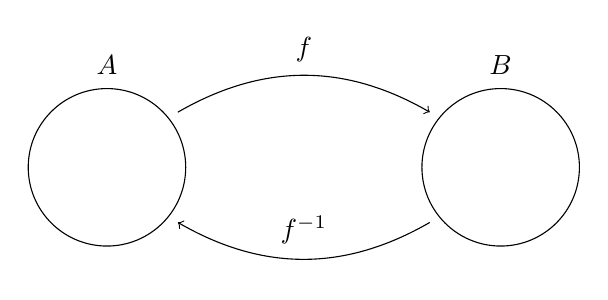
\begin{tikzpicture}
		\draw (0,0) circle (1cm);
		\draw (5,0) circle (1cm);
		\draw[-{To[scale = 1.3]}] (0.9,0.7)	to[out = 30, in = 150] (4.1,0.7);
		\draw[-{To[scale = 1.3]}] (4.1,-0.7)	to[out = -150, in = -30] (0.9,-0.7);
		\node at (0,1.3) {$A$};
		\node at (5,1.3) {$B$};
		\node at (2.5,1.5) {$f$};
		\node at (2.5,-0.8) {$f^{-1}$};
	\end{tikzpicture}
	\caption{Funktion $f$ samt invers funktion $f^{-1}$.}
	\label{fig:inv}
\end{figure}
\begin{exa}
Funktionen $f: \mathbb{R} \to \mathbb{R}$ givet ved
\begin{align*}
	f(x) = 4x+7
\end{align*}
er bijektiv. Vi kan finde den inverse funktion til $f$ ved at isolere $x$ i ligningen
\begin{align*}
	y = 4x+7 \ \Leftrightarrow \ y-7 = 4x \ \Leftrightarrow \frac{y-7}{4} = x.
\end{align*}
Derfor er funktionen $f^{-1}:\mathbb{R} \to \mathbb{R}$ givet ved
\begin{align*}
	f^{-1}(x) = \frac{x-7}{4}
\end{align*}
den inverse funktion til $f$. Vi kan tjekke dette ved at bestemme den sammensatte funktion $f\circ f^{-1}$:
\begin{align*}
f\circ f^{-1}(x) &= f^{-1}(f(x))\\
&= \frac{4x+7-7}{4}\\
&= \frac{4x}{4}\\
&= x.
\end{align*}
\end{exa}

\begin{exa}
Hvis vi betragter kvadratfunktionen $f: \mathbb{R}_{\geq 0} \to \mathbb{R}_{\geq 0}$ givet ved
\begin{align*}
	f(x) = x^2
\end{align*}
til første kvadrant, så har den kvadratrodsfunktionen $f^{-1}: \mathbb{R}_{\geq 0} \to \mathbb{R}_{\geq 0}$ udtrykt ved
\begin{align*}
	f^{-1}(x) = \sqrt{x}
\end{align*}
som invers funktion, siden
\begin{align*}
	\sqrt{x^2} = x.
\end{align*}
\end{exa}

\subsection*{Opgave 1}
Afgør, hvilke af følgende der er surjektive, injektive eller bijektive. I fald de er bijektive, bestem så den inverse funktion. 
\begin{center}
\begin{tikzpicture}
	\node at (1,0.6) {$f$};
	\node at (0,0) (1) {$a$};
	\node at (0,-1) (2) {$b$};
	\node at (0,-2) (3) {$c$};
	\node at (0,-3) (4) {$d$};
	\node at (2,0) (5) {$2$};
	\node at (2,-1) (6) {4};
	\node at (2,-2) (7) {6};
	\draw[-{To[scale = 1.3]}] (1) -- (5);
	\draw[-{To[scale = 1.3]}] (2) -- (6);
	\draw[-{To[scale = 1.3]}] (3) -- (7);
	\draw[-{To[scale = 1.3]}] (4) -- (6);
	\node at (6,0.6)  {$f$};
	\node at (5,0) (10) {$1$};
	\node at (5,-1) (20) {$2$};
	\node at (7,-0) (30) {1};
	\node at (7,-1) (40) {2};
	\node at (7,-2) (50) {3};
	\node at (7,-3) (60) {4};
	\draw[-{To[scale = 1.3]}] (10) -- (30);
	\draw[-{To[scale = 1.3]}] (20) -- (50);
\end{tikzpicture}\\
\vspace{1cm}
\begin{tikzpicture}
	\node at (1,0.6)  {$f$};
	\node at (0,0) (1) {$\alpha$};
	\node at (0,-1) (2) {$\beta$};
	\node at (0,-2) (3) {$\zeta$};
	\node at (2,0) (4) {$a$};
	\node at (2,-1) (5) {$b$};
	\node at (2,-2) (6) {$c$};
	\draw[-{To[scale = 1.3]}] (1) -- (4);
	\draw[-{To[scale = 1.3]}] (2) -- (5);
	\draw[-{To[scale = 1.3]}] (3) -- (6);
	\node at (6,0.6)  {$f$};
	\node at (5,0) (10) {$-3$};
	\node at (5,-1) (20) {$-2$};
	\node at (5,-2) (30) {$-1$};
	\node at (5,-3) (40) {$0$};
	\node at (5,-4) (50) {$1$};
	\node at (5,-5) (60) {$2$};
	\node at (5,-6) (70) {$3$};
	\node at (7,0) (80) {3};
	\node at (7,-1) (90) {2};
	\node at (7,-2) (100) {1};
	\node at (7,-3) (110) {0};
	\draw[-{To[scale = 1.3]}] (10) -- (80);
	\draw[-{To[scale = 1.3]}] (20) -- (90);
	\draw[-{To[scale = 1.3]}] (30) -- (100);
	\draw[-{To[scale = 1.3]}] (40) -- (110);
	\draw[-{To[scale = 1.3]}] (50) -- (100);
	\draw[-{To[scale = 1.3]}] (60) -- (90);
	\draw[-{To[scale = 1.3]}] (70) -- (80);			
\end{tikzpicture}\\
\vspace{1cm}
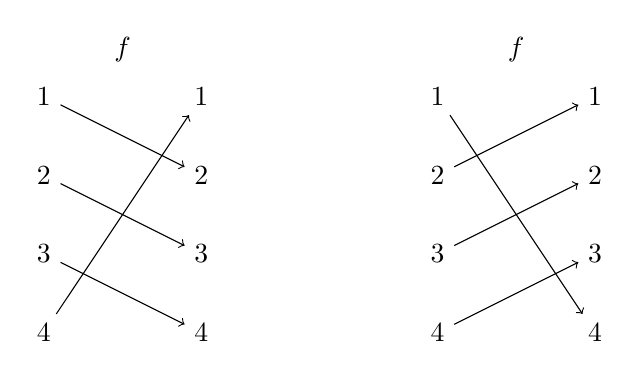
\begin{tikzpicture}
	\node at (1,0.6) {$f$};
	\node at (0,0) (1) {$1$};
	\node at (0,-1) (2) {$2$};
	\node at (0,-2) (3) {$3$};
	\node at (0,-3) (4) {$4$};
	\node at (2,0) (5) {1};
	\node at (2,-1) (6) {2};
	\node at (2,-2) (7) {3};
	\node at (2,-3) (8) {4};
	\draw[-{To[scale = 1.3]}] (1) -- (6);
	\draw[-{To[scale = 1.3]}] (2) -- (7);
	\draw[-{To[scale = 1.3]}] (3) -- (8);
	\draw[-{To[scale = 1.3]}] (4) -- (5);
	\node at (6,0.6)  {$f$};
	\node at (5,0) (10) {$1$};
	\node at (5,-1) (20) {$2$};
	\node at (5,-2) (30) {$3$};
	\node at (5,-3) (40) {$4$};
	\node at (7,0) (50) {1};
	\node at (7,-1) (60) {2};
	\node at (7,-2) (70) {3};
	\node at (7,-3) (80) {4};
	\draw[-{To[scale = 1.3]}] (10) -- (80);
	\draw[-{To[scale = 1.3]}] (20) -- (50);
	\draw[-{To[scale = 1.3]}] (30) -- (60);
	\draw[-{To[scale = 1.3]}] (40) -- (70);
\end{tikzpicture}
\end{center}


\subsection*{Opgave 2}
I følgende opgaver kan det være en fordel at tegne funktionerne.
\begin{enumerate}[label=\roman*)]
	\item Funktionen $f:\mathbb{R} \to \mathbb{R}$ er givet ved
	\begin{align*}
		f(x) = 10x.
	\end{align*}
	Afgør, om $f$ er surjektiv, injektiv eller bijektiv. 
	\item Funktionen $f:\mathbb{R} \to \mathbb{R}$ er givet ved
	\begin{align*}
		f(x) = x^3.
	\end{align*}
	Afgør, om $f$ er surjektiv, injektiv eller bijektiv. 
	\item Funktionen $f:\mathbb{R} \to \mathbb{R}$ er givet ved
	\begin{align*}
		f(x) = x^2-3x+7.
	\end{align*}
	Afgør, om $f$ er surjektiv, injektiv eller bijektiv. 
	\item Funktionen $f:\mathbb{R} \to \mathbb{R}$ er givet ved
	\begin{align*}
		f(x) = 2x^3-5x^2-2.
	\end{align*}
	Afgør, om $f$ er surjektiv, injektiv eller bijektiv. 
\end{enumerate}


\subsection*{Opgave 3}
\begin{enumerate}[label=\roman*)]
	\item Lad $A$ bestå af alle varer i et supermarked. En funktion $f:A \to \mathbb{R}$ giver prisen på varen. 
	Er funktionen surjektiv, injektiv eller bijektiv?
	\item Lad $A$ være alle elever på Nørre. Funktionen $f:A \to \{15,16,17,18,19,20,21\}$ giver alderen på en elev. Er funktionen surjektiv, injektiv eller bijektiv?
	\item Lad $A$ betegne mængden af alle danskere og $B$ betegner mængden af alle CPR-numre. Funktionen $f:A \to B$ giver CPR-nummeret på en person. Er funktionen surjektiv, injektiv eller bijektiv? 
\end{enumerate}

\subsection*{Opgave 4}
\begin{enumerate}[label=\roman*)]
	\item Afgør om funktionen $f: ]-2,3] \to [1,3[$ givet ved følgende graf er surjektiv, injektiv eller bijektiv.
	\begin{center}
\resizebox{0.45\textwidth}{!}{
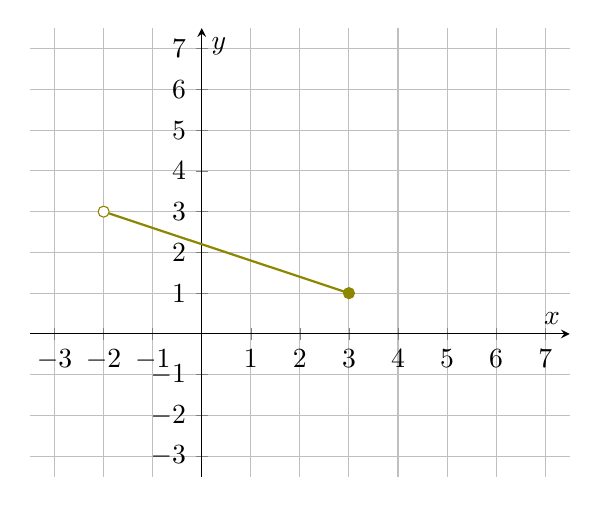
\begin{tikzpicture}
	\begin{axis}
	[axis lines = center, 
	xmin = -3.5, xmax = 7.5,
	ymin = -3.5, ymax = 7.5,
	grid = both,
	xtick = {-3,-2,...,6,7},
	ytick = {-3,-2,...,6,7},
	xlabel = $x$, ylabel = $y$
	]
		\addplot[color = olive, thick, domain = -2:3] {-2/5*x+2.2};	
		\filldraw[color = white](axis cs: -2,3) circle (2pt);
		\filldraw[color = olive](axis cs: 3,1) circle (2pt);
		\draw[color = olive](axis cs: -2,3) circle (2pt);
	\end{axis}
\end{tikzpicture}
}
\end{center}

\item Afgør om funktionen $f: [-1,4[ \to [0,16[$ givet ved følgende graf er surjektiv, injektiv eller bijektiv.
	\begin{center}
		\resizebox{0.45\textwidth}{!}{
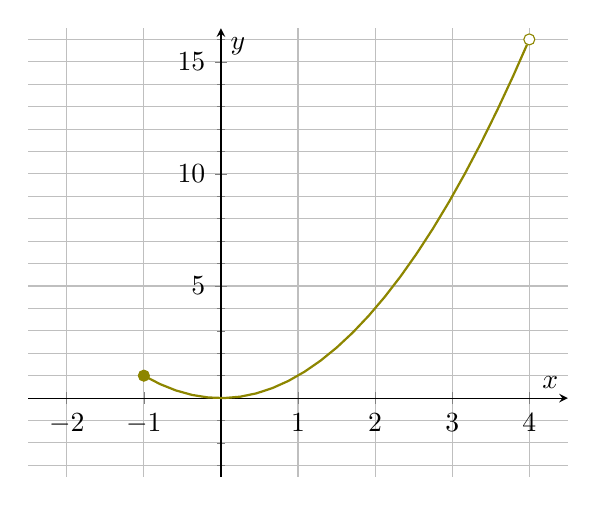
\begin{tikzpicture}
	\begin{axis}
	[axis lines = center, 
	xmin = -2.5, xmax = 4.5,
	ymin = -3.5, ymax = 16.5,
	xtick = {-3,-2,...,4,5},
	ytick = {-5,0,...,15,20},
	minor y tick num = 4,
	grid = both,
	xlabel = $x$, ylabel = $y$,
	]
		\addplot[color = olive, thick, domain = -1:4] {x^2};	
		\filldraw[color = white](axis cs: 4,16) circle (2pt);
		\filldraw[color = olive](axis cs: -1,1) circle (2pt);
		\draw[color = olive](axis cs: 4,16) circle (2pt);	
	\end{axis}
\end{tikzpicture}
}	
	\end{center}

\item Afgør om funktionen $f: ]1,6[ \to ]1,4]$ givet ved følgende graf er surjektiv, injektiv eller bijektiv.
\begin{center}
	\resizebox{0.45\textwidth}{!}{
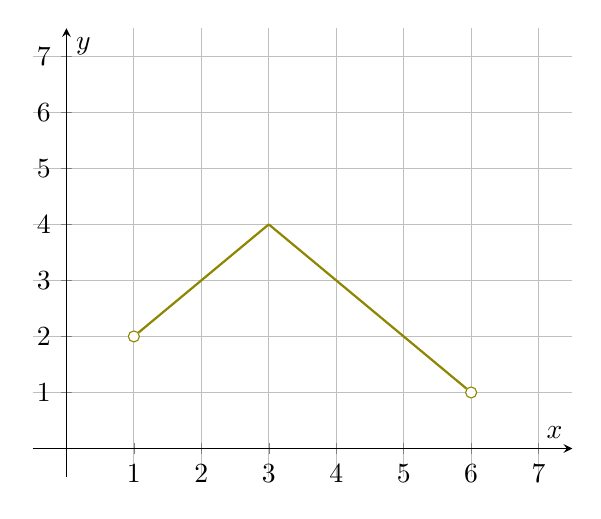
\begin{tikzpicture}
	\begin{axis}
	[axis lines = center, 
	xmin = -0.5, xmax = 7.5,
	ymin = -0.5, ymax = 7.5,
	grid = both,
	xtick = {-3,-2,...,6,7},
	ytick = {-3,-2,...,6,7},
	xlabel = $x$, ylabel = $y$
	]
		\addplot[color = olive, thick, domain = 1:3] {x + 1};
		\addplot[color = olive, thick, domain = 3:6] {-x + 7};	
		\filldraw[color = white](axis cs: 1,2) circle (2pt);
		\filldraw[color = white](axis cs: 6,1) circle (2pt);
		\draw[color = olive](axis cs: 1,2) circle (2pt);
		\draw[color = olive](axis cs: 6,1) circle (2pt);
	\end{axis}
\end{tikzpicture}
}
\end{center}
\item Afgør om funktionen $f: [-7,7[ \to [-1,1]$ givet ved følgende graf er surjektiv, injektiv eller bijektiv.
\begin{center}
	\resizebox{0.45\textwidth}{!}{
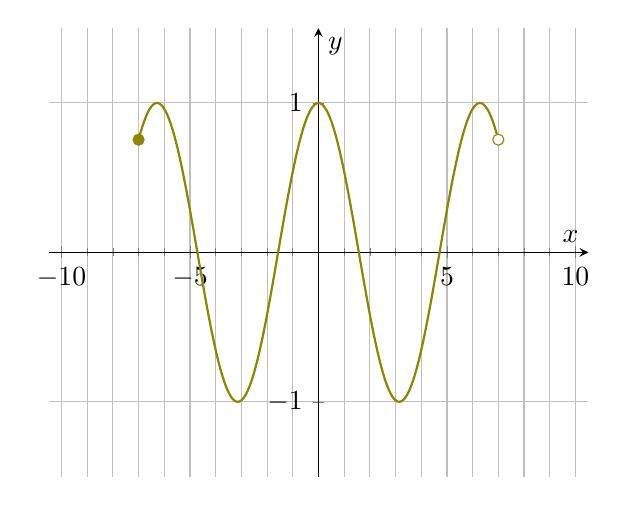
\begin{tikzpicture}
	\begin{axis}
	[axis lines = center, 
	xmin = -10.5, xmax = 10.5,
	ymin = -1.5, ymax = 1.5,
	grid = both,
	xtick = {-15,-10,...,10,15},
	minor x tick num = 4,
	ytick = {-1,0,1},
	xlabel = $x$, ylabel = $y$
	]
		\addplot[color = olive, thick, domain = -7:7, samples = 200] {cos(deg(x))};	
		\filldraw[color = white](axis cs: 7,0.754) circle (2pt);
		\filldraw[color = olive](axis cs: -7,0.754) circle (2pt);
		\draw[color = olive](axis cs: 7,0.754) circle (2pt);
	\end{axis}
\end{tikzpicture}
}
\end{center}

\end{enumerate}
\subsection*{Opgave 5}
\begin{enumerate}[label=\roman*)]
	\item Funktionen $f:\mathbb{R} \to \mathbb{R}$ givet ved 
	\begin{align*}
		f(x) = 3x+1
	\end{align*}
	er bijektiv. Bestem en invers funktion $f^{-1}:\mathbb{R} \to \mathbb{R}$ til $f$. 
	\item Funktionen $f:\mathbb{R} \to \mathbb{R}$ givet ved 
	\begin{align*}
		f(x) = -7x-13
	\end{align*}
	er bijektiv. Bestem en invers funktion $f^{-1}:\mathbb{R} \to \mathbb{R}$ til $f$. 
	\item Funktionen $f:\mathbb{R} \to \mathbb{R}$ givet ved 
	\begin{align*}
		f(x) = x^3
	\end{align*}
	er bijektiv. Bestem en invers funktion $f^{-1}:\mathbb{R} \to \mathbb{R}$ til $f$. 
\end{enumerate}

\subsection*{Opgave 6}
\begin{enumerate}[label=\roman*)]
	\item Afgør, om funktionerne $f$ og $g$ givet ved henholdsvis 
	\begin{align*}
		f(x) &= \frac{\log_2(x)+6}{4},\\
		g(x) &= 2^{4x - 6}.
	\end{align*}
	er hinandens inverse
	\item Afgør, om funktionerne $f$ og $g$ givet ved henholdsvis
	\begin{align*}
		f(x) &= (5x-7)^3,\\
		g(x) &= \frac{\sqrt[3]{x}+7}{3}.
	\end{align*}
	er hinandens inverse.
\end{enumerate}